\section{Simulação da Partida Direta a Vazio ($T_L = 0$)}\label{sec:partida_vazio}

A energização direta com o eixo desprovido de carga resistente mecânica externa ($T_L = 0$) submete os enrolamentos estatóricos à máxima solicitação eletrodinâmica durante o intervalo de aceleração da pesada inércia acoplada da bancada. A simulação dinâmica no Simscape SPS viabiliza confrontar o envelope de amortecimento da corrente de \textit{inrush} com a dedução teórica a rotor bloqueado e inspecionar a acomodação no regime permanente a vazio.

% =========================================================================
% [DIRETRIZ DE REDAÇÃO]
% - Objetivo: Atender ao Item 2.C de sim_proj.pdf. Simular a partida direta a vazio (T_L = 0)
%   e demonstrar com gráficos que a corrente atinge o pico previsto e converge para o regime a vazio.
% - Formulação: Analisar o tempo de aceleração prolongado (~1,5 s) decorrente da inércia
%   pesada acoplada (J = 0,701 kg*m^2), o conjugado pulsante inicial e o escorregamento residual a vazio.
% - Figuras/Tabelas: Incluir os 3 gráficos do transitório de partida a vazio:
%   item2c_transient_dol_current.png, item2c_transient_dol_speed.png e item2c_transient_dol_torque.png.
% - Confronto: Confrontar o pico medido na simulação (105,7 A) com o inrush teórico deduzido
%   no Item 2.B, e a corrente eficaz a vazio simulada (7,55 A) com a previsão analítica.
% =========================================================================

\subsection{Comportamento da Corrente de Estator e Validação de Inrush}\label{subsec:partida_corrente}

A \Cref{fig:partida_corrente} exibe a forma de onda temporal da corrente instantânea de linha no estator durante o período de aceleração.

\begin{figure}[H]
\centering
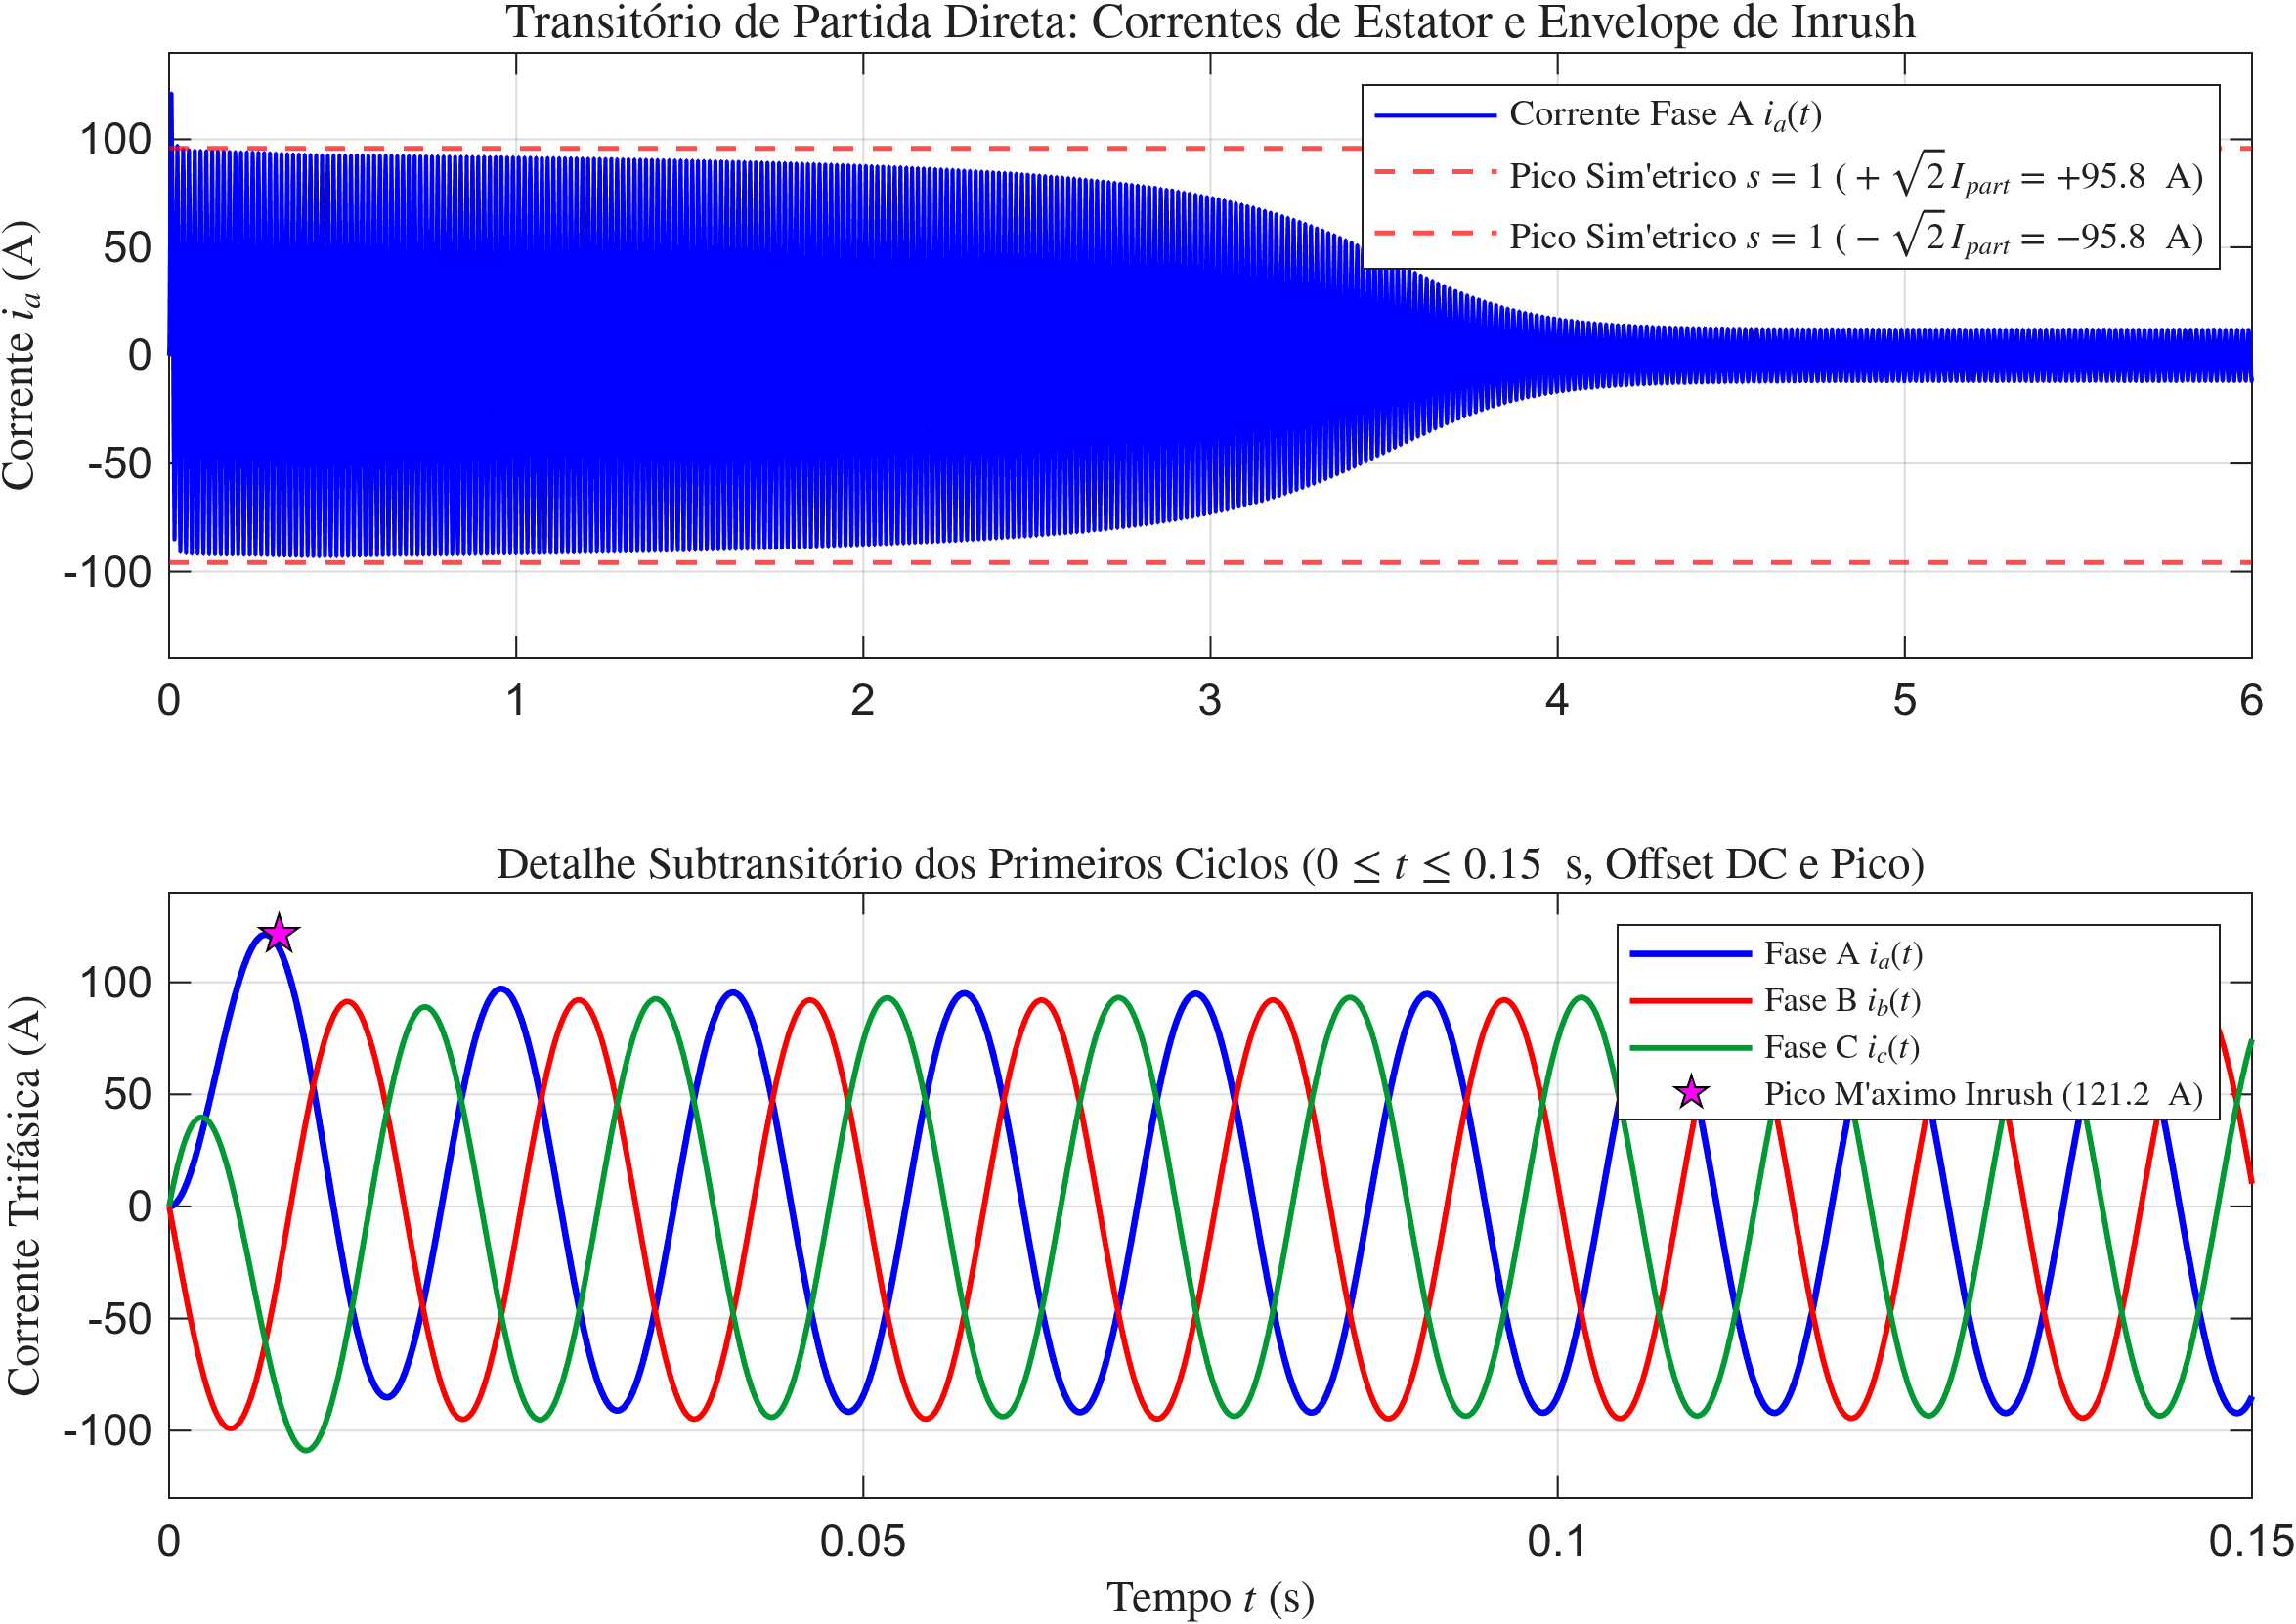
\includegraphics[width=0.82\textwidth]{item2c_transient_dol_current.png}
\caption{Transitório da Corrente de Linha de Estator durante a partida direta a vazio ($T_L = 0$).}
\label{fig:partida_corrente}
\end{figure}

O pico máximo registrado atinge $I_{peak} = \SI{105,7}{\ampere}$, compreendido entre a crista simétrica ($\sqrt{2} \cdot I_{line,cc} = \SI{96,32}{\ampere}$) e o limite superior assimétrico teórico ($I_{peak,teorico} = \SI{119,6}{\ampere}$), validando o modelo dinâmico frente à formulação analítica do Item 2.B. Após \SI{1,5}{\second}, a corrente estabiliza em $I_0 = \SI{7,55}{\ampere}$ eficazes.

\subsection{Dinâmica de Velocidade e Conjugado Eletromagnético}\label{subsec:partida_velocidade_torque}

As \Cref{fig:partida_velocidade,fig:partida_torque} ilustram a trajetória de aceleração angular e as oscilações eletromecânicas iniciais de conjugado.

\begin{figure}[H]
\centering
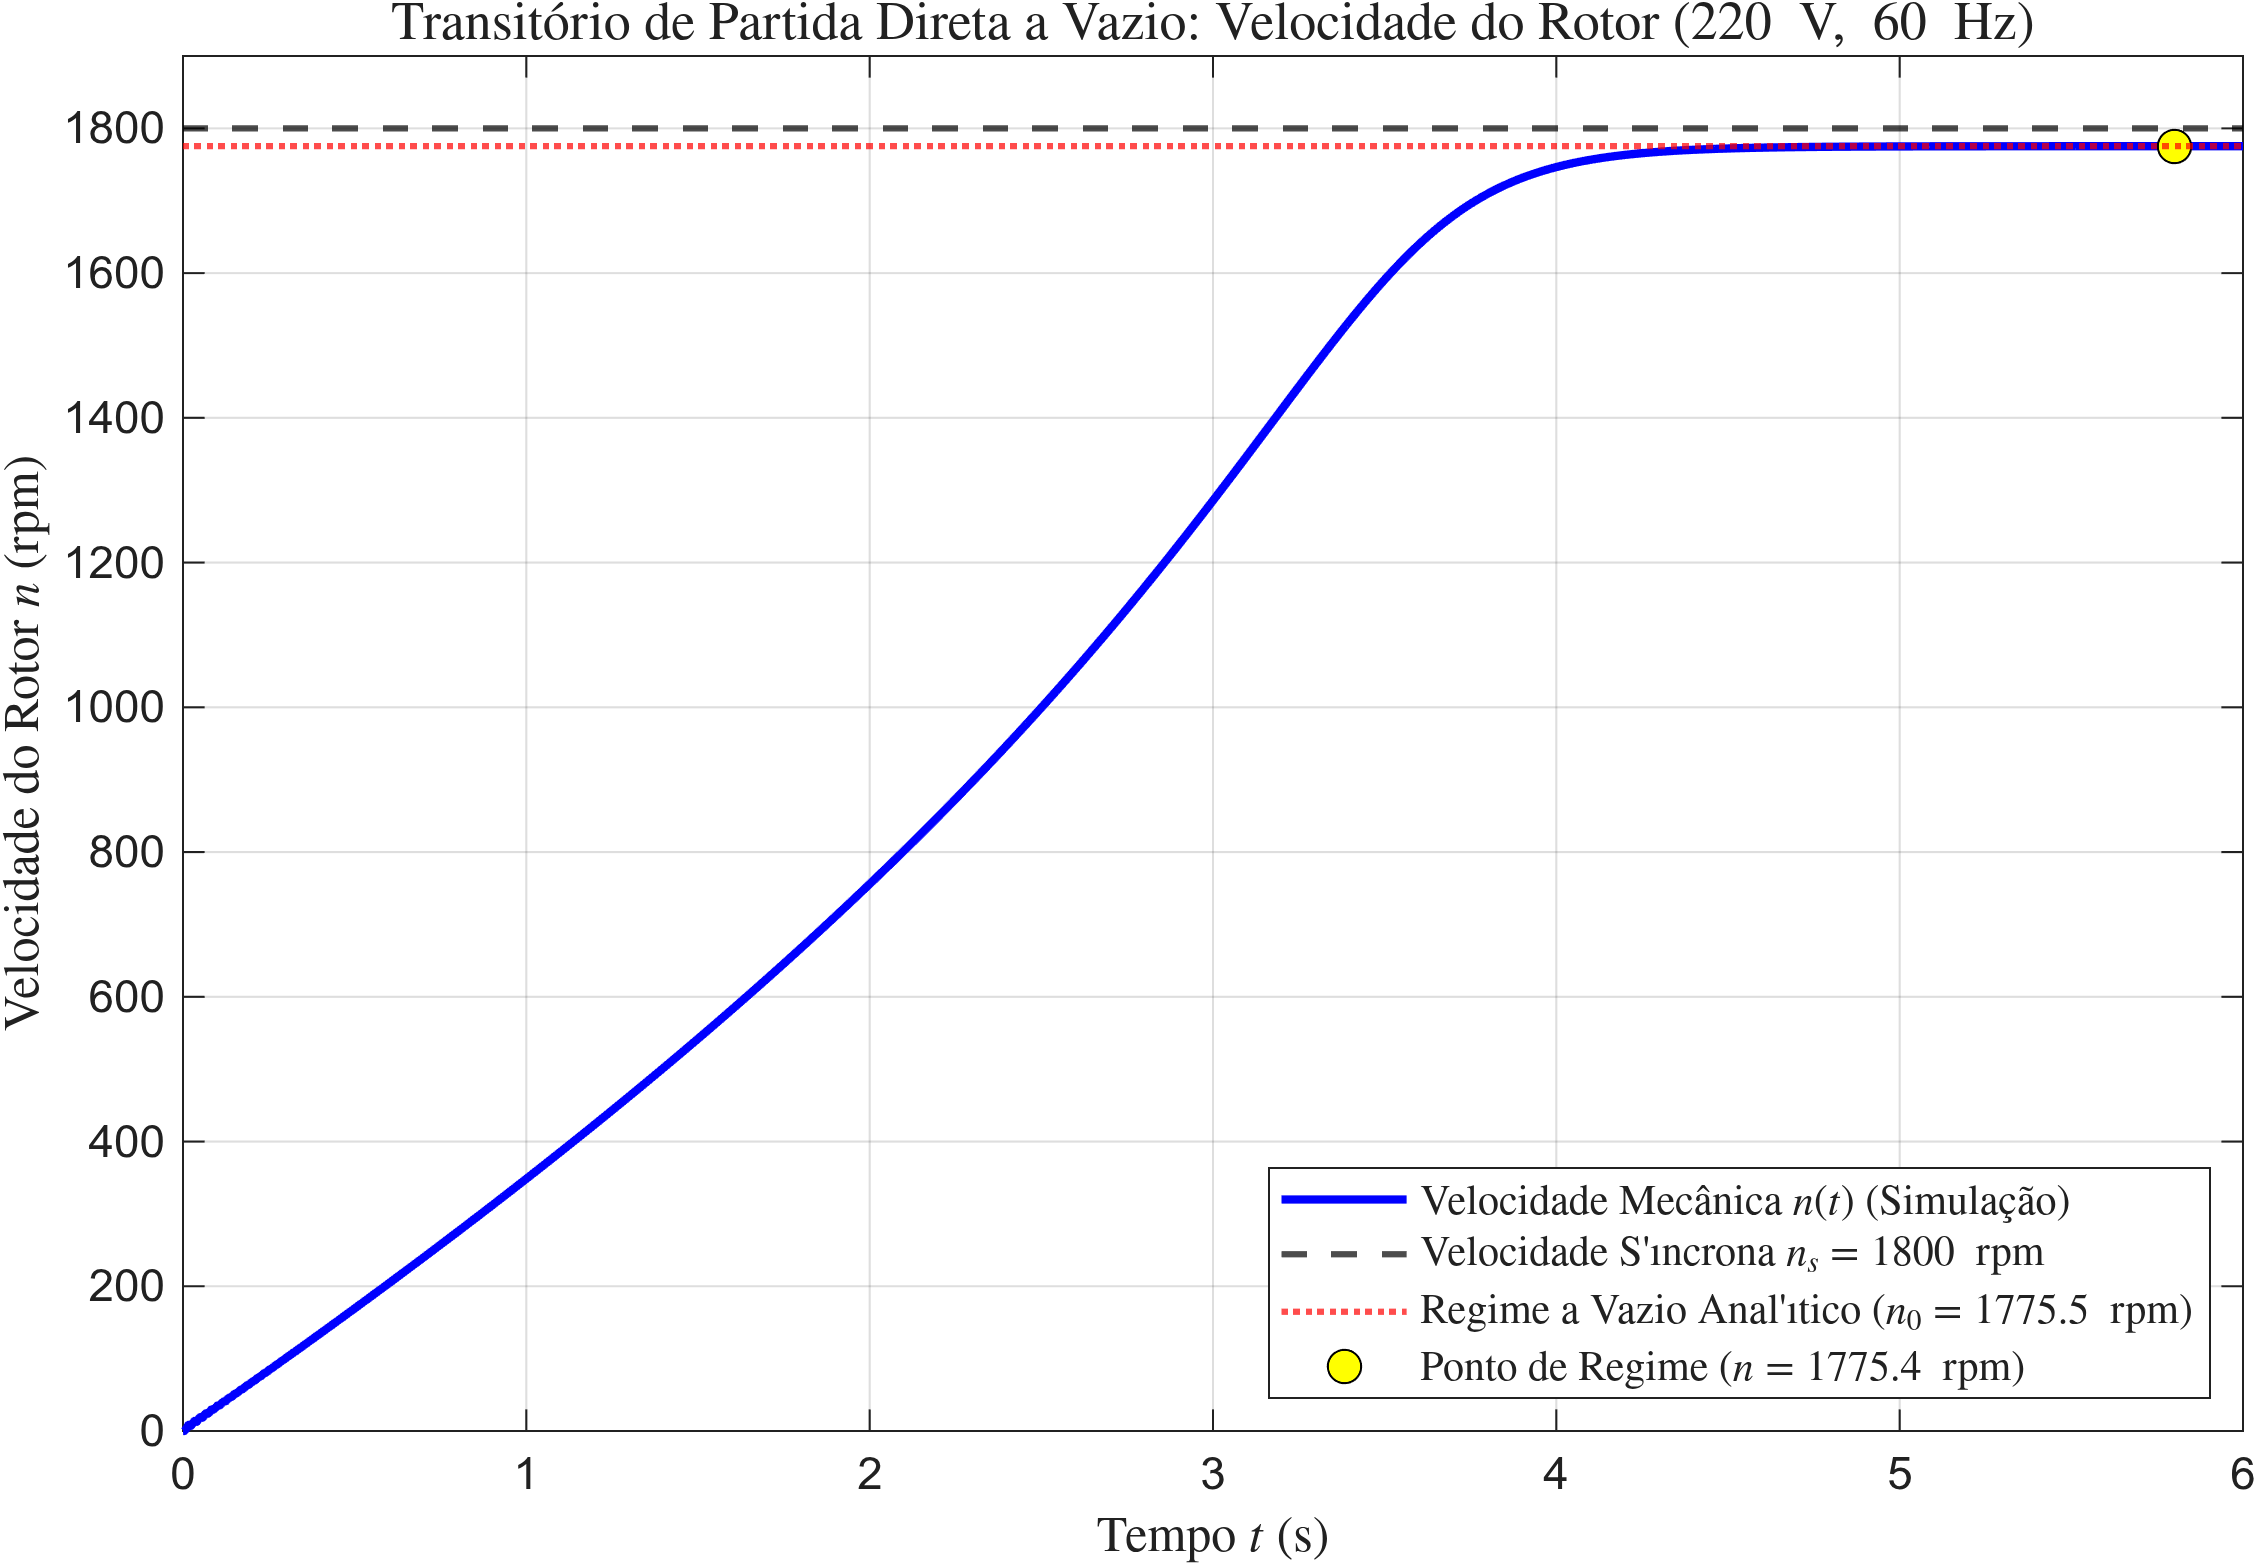
\includegraphics[width=0.82\textwidth]{item2c_transient_dol_speed.png}
\caption{Trajetória temporal de aceleração da Velocidade do Rotor durante a partida direta a vazio.}
\label{fig:partida_velocidade}
\end{figure}

\begin{figure}[H]
\centering
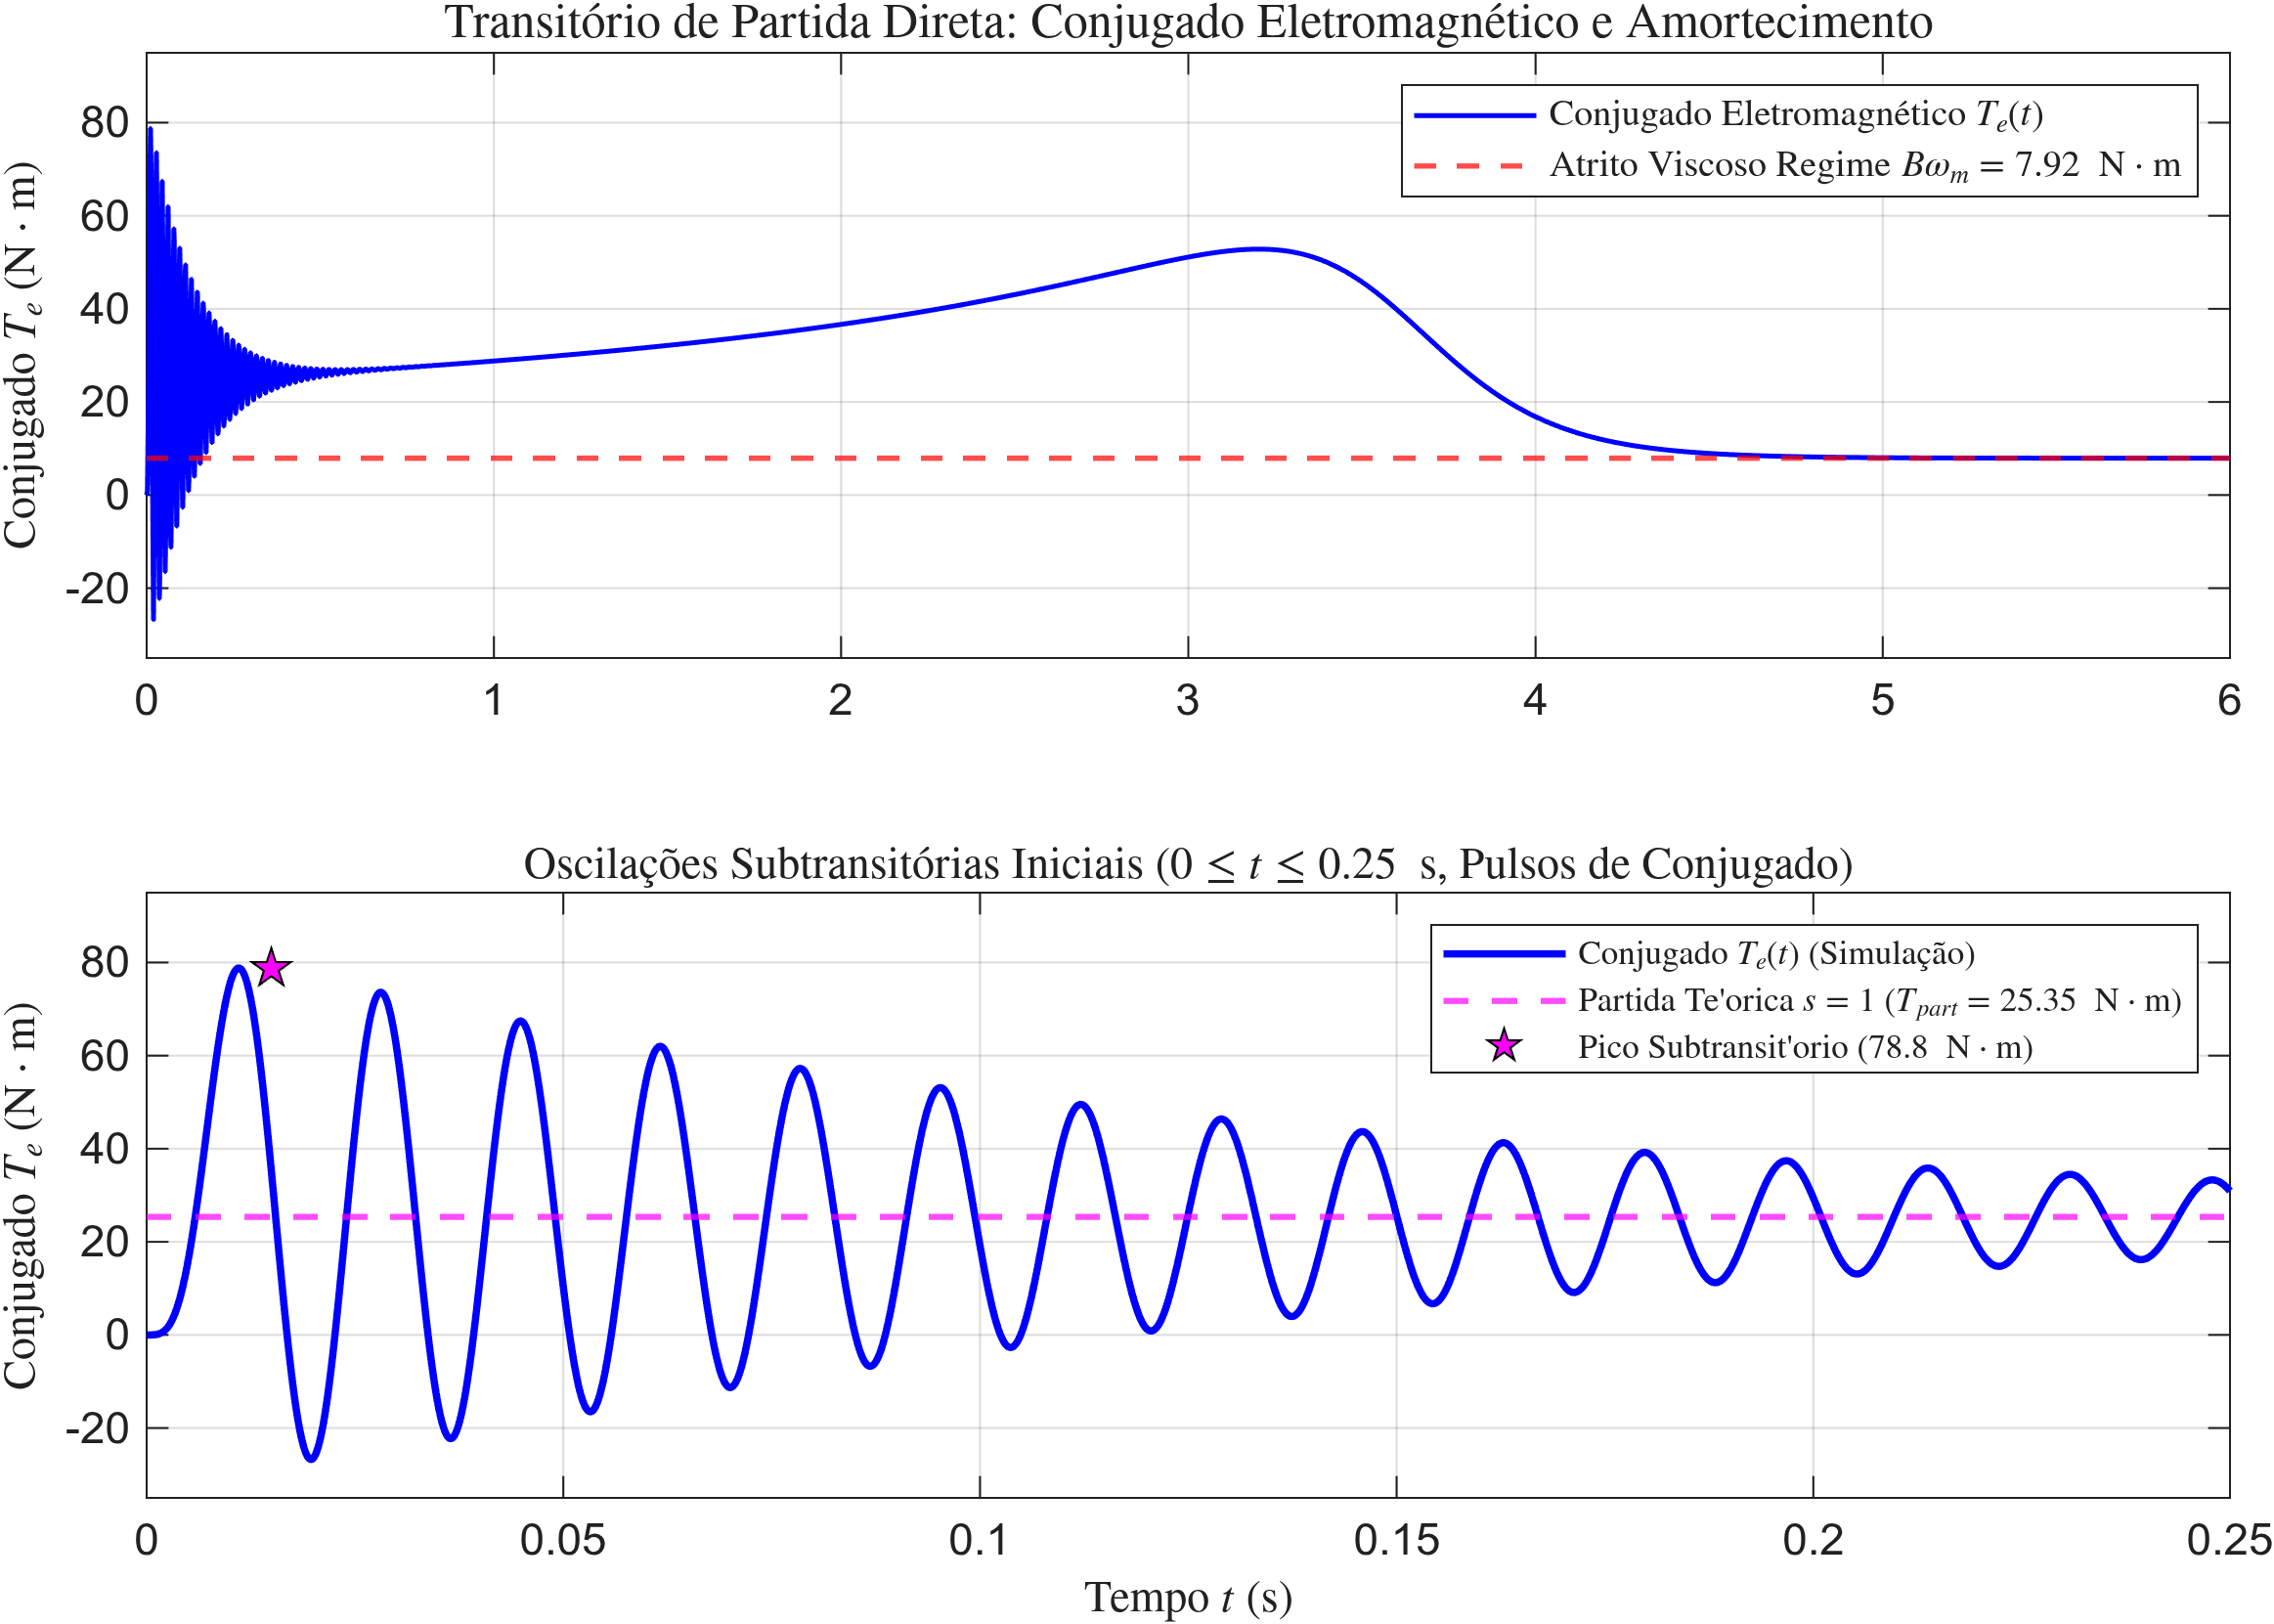
\includegraphics[width=0.82\textwidth]{item2c_transient_dol_torque.png}
\caption{Transitório do Conjugado Eletromagnético durante a partida direta a vazio.}
\label{fig:partida_torque}
\end{figure}

A resposta de velocidade reflete a inércia acoplada ($J = \SI{0,701}{\kilogram\meter\squared}$), com acomodação em $n_0 = \SI{1797,0}{\RPM}$ ($s \approx 0{,}0016$), enquanto o conjugado oscila inicialmente entre $-\SI{20}{\Nm}$ e $+\SI{60}{\Nm}$ até equilibrar as perdas por atrito viscoso ($T_{friction} = B\omega_m \approx \SI{8,0}{\Nm}$).
